\documentclass[tikz]{standalone}

\usepackage[utf8]{inputenc}
\usepackage[T1]{fontenc}
\usepackage{cmap}
\usepackage{amsmath}
\usepackage{amssymb}
\usepackage{verbatim}
\usepackage{bm}
\usepackage{siunitx}

\renewcommand{\familydefault}{\sfdefault}
\usepackage[cm]{sfmath}

\usepackage{tikz}
\usetikzlibrary{math}
\usetikzlibrary{bending}
\usetikzlibrary{decorations.pathreplacing}
\usetikzlibrary{decorations.pathmorphing}
\usetikzlibrary{fadings}
\usetikzlibrary{positioning}
\definecolor{cblue}{rgb}{0.396, 0.643, 0.82}
\definecolor{corange}{rgb}{1.0, 0.69, 0.416}
\definecolor{cgreen}{rgb}{0.471, 0.824, 0.471}
\definecolor{cred}{rgb}{1.0, 0.502, 0.502}
\definecolor{cpurple}{rgb}{0.863, 0.78, 0.937}

\def\symbhwaas{N_a}
\def\symbsteplen{\Delta d}
\def\symbsweeprate{f_s}
\def\symbsweepperiod{T_s}
\def\symbsweepdur{\tau_s}
\def\symbframerate{f_f}
\def\symbframeperiod{T_f}
\def\symbframedur{\tau_f}
\def\symbprf{f_\text{p}}
\def\symbspf{N_s}
\def\symbstartpoint{d_1}
\def\symbnumpoints{N_d}
\def\symbmur{r_\text{u}}
\def\symbcid{r_\ell}
\def\symbminmd{r_\text{min}}
\def\symbmaxmd{r_\text{max}}
\def\symbdcrnear{r_\text{near}}
\def\symbdcrfar{r_\text{far}}

\begin{document}

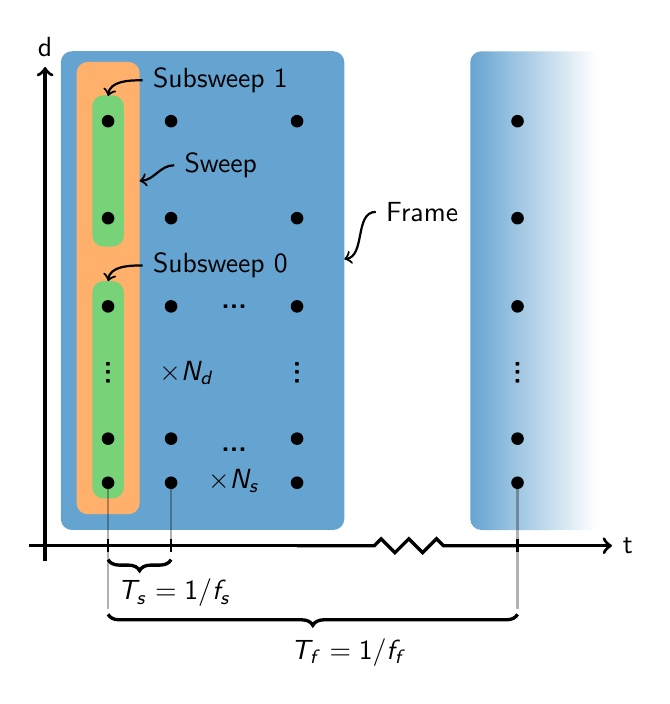
\begin{tikzpicture}[scale=0.8]
  \tikzmath{
    \ph = 0.7;
    %
    \nump = 5;
    \numpTwo = 2;
    \startp = 20;
    \steplen = 3;
  }

  % x-axis
  \draw [very thick] (-0.25, 0) -- (4, 0);
  \draw [very thick, decoration=straight zigzag, decorate] (4, 0) -- (7.5, 0);
  \draw [->, very thick] (7.5, 0) -- (9, 0) node[right]{t};
  % y-axis
  \draw [->, very thick] (0, -0.25) -- (0, {(\nump + \numpTwo + 1)*\ph+2}) node[above]{d};

  % sweep and frame boxes
  \fill [fill=cblue, rounded corners] (0.25, 0.25) rectangle ++(4.5, {(\nump+ \numpTwo)*\ph+2.7});
  \fill [fill=corange, rounded corners] (0.5, 0.5) rectangle ++(1, {(\nump+\numpTwo+.4)*\ph+2});
  \fill [fill=cgreen, rounded corners] (0.75, 0.75) rectangle ++(.5, {(\nump-1.5)*\ph+1});
  \fill [fill=cgreen, rounded corners] (0.75, 4.75) rectangle ++(.5, {(\numpTwo)*\ph+1});
  \fill [fill=cblue, rounded corners, path fading=east] (8.75, 0.25) -- ++(-2, 0) -- ++(0, {(\nump+ \numpTwo)*\ph+2.7}) -- ++(2, 0);

  % sweep and frame labels
  \draw [<-, thick] (1, {(\nump-1)*\ph+1.4}) to [out=90, in=180] ++(0.55, 0.25) node [right] {Subsweep 0};
  \draw [<-, thick] (1, {(\nump + \numpTwo +1.2)*\ph+1.4}) to [out=90, in=180] ++(0.55, 0.25) node [right] {Subsweep 1};
  \draw [<-, thick] (1.5, {(\nump + 2.7)*\ph+0.4}) to [out=0, in=180] ++(0.55, 0.25) node [right] {Sweep};
  \draw [<-, thick] (4.75, {(\nump-1)*\ph+1.75}) to [out=0, in=180] ++(0.5, 0.75) node [right] {Frame};

  % points
  \foreach \i in {1, 2, 5} {
    \tikzmath{
      \y = \i - 1;
      int \ytext;
      \ytext = (\i-1)*\steplen + \startp;
      \yy = \y*\ph;
    }
    \foreach \x in {0, 1, 3, 6.5} {
      \fill [fill=black] (\x + 1, \yy + 1) circle (1mm);
    }
  }

  \foreach \i in {7, 9.2} {
    \tikzmath{
      \y = \i - 1;
      int \ytext;
      \yy = \y*\ph;
    }
    \foreach \x in {0, 1, 3, 6.5} {
      \fill [fill=black] (\x + 1, \yy + 1) circle (1mm);
    }
  }

  \foreach \x in {0, 3, 6.5} {
    \node[rotate=90] at (\x + 1, {2.5*\ph+1}) {$\bm\ldots$};
  }

  \node at (2.25, {2.5*\ph+1}) {$\times \symbnumpoints$};

  % repeat for number of sweeps
  \node at (3, {0.5*(2.5-1)*\ph+1}) {$\bm\ldots$};
  \node at (3, {4*\ph+1}) {$\bm\ldots$};
  \node at (3, {0.5*(2.5-1)*\ph+0.5}) {$\times \symbspf$};

  % x ticks
  \foreach \x in {1, 2, 7.5} {
      \draw [thick] (\x, 0.1) -- ++(0, -0.2);
  }

  % x lines
  \draw [thick, opacity=0.3] (1, 1) -- (1, -1);
  \draw [thick, opacity=0.3] (7.5, 1) -- ++(0, -2);
  \draw [thick, opacity=0.3] (2, 1) -- (2, 0);

  % x curlys
  \draw [very thick, decoration={brace, amplitude=4pt, mirror, raise=5pt}, decorate] (1, 0) -- (2, 0);
  \node [right] at (1, -0.75) {$\symbsweepperiod = 1/\symbsweeprate$};

  \draw [very thick, decoration={brace, amplitude=4pt, mirror, raise=2pt}, decorate] (1, -1.0) -- (7.5, -1.0);
  \node [right] at (3.75, -1.7) {$\symbframeperiod = 1/\symbframerate$};
\end{tikzpicture}

\end{document}
